% 1. Submission Content
\chapter{Approach Outline}

    % 1.1 Problem Understanding
    \section{Problem Understanding}
    \subsection{Summary of Problem}
    Provide a brief summary of the single motor failure problem. Explain the specific challenges in maintaining stability and control with a failed motor.

    \subsection{Challenges}
    \begin{itemize}
        \item Reduced thrust and control with only three functioning motors.
        \item Asymmetric thrust distribution impacting stability.
        \item Complications in both hover stability and landing.
    \end{itemize}

    % 1.2 Solution Overview
    \section{Solution Overview}
    \subsection{Control Algorithm Design}
    Outline the control algorithm, including core concepts like the recovery mechanism and assumptions made.

    \subsection{Recovery Approach}
    Describe the initial recovery strategy to mitigate the effects of a single motor failure. This could include techniques like rebalancing thrust among the remaining motors or adjusting pitch and yaw controls.

    % 1.3 Background Study
    \section{Background Study}
    Mention the relevant literature, research articles, or technical papers you reviewed to inform your approach. Cite them properly.

    % 1.4 Images and Tables 
    \section{Images \& Tables}
    This section is just for your reference.
    \subsection{Images}
    This is a figure.\\
    \begin{figure}[h!]      % The h! here makes sure that the image stays where you have put, else Latex has a habit to move shit around according to its will
        \centering
        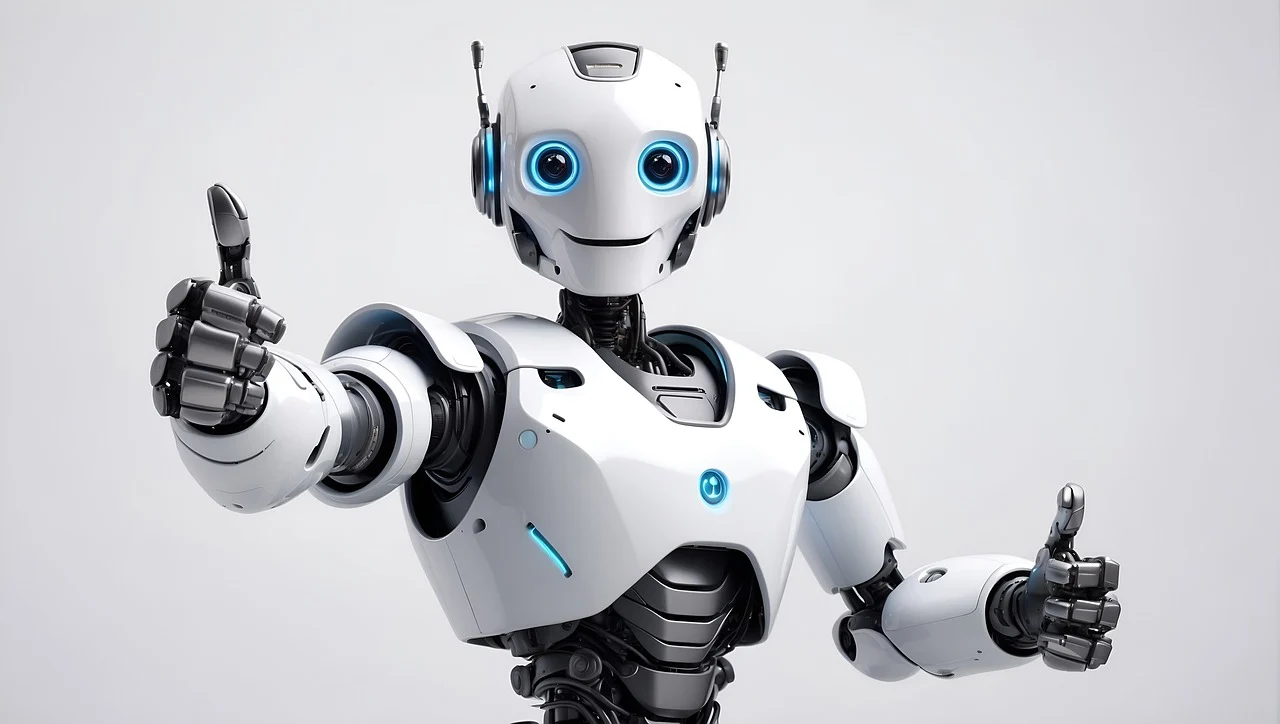
\includegraphics[width=0.7\textwidth]{images/example_image.jpg}
        \caption{Example of quadrotor stability during motor failure scenario.}
        \label{fig:example image}
    \end{figure}
    
    \subsection{Tables}
    \begin{table}[h]
        \centering
        \begin{tabular}{|c|c|}      % Each pipe shows a vertical line
            \hline      % Makes the horizontal line
            (0, 0) & (0, 1)\\
            \hline
            (1, 0) & (1, 1) \\
            \hline
        \end{tabular}
        \caption{Caption}
        \label{tab:my_label}
    \end{table}

    In case your table is something huge ass and doesn't fit in the page, do not worry, use ChatGPT, if it can't do (which I assume should not be the case), then simply opt for "long table", also this function can be used for a multi-page table, but I am assuming we do not have that.